\documentclass{article}
\usepackage{tikz}

\usetikzlibrary{arrows,decorations.markings}

\title{Computer Science - Architecture and Organization Notes}
\author{Conrad A. Mearns}

\begin{document}

\maketitle

\noindent
\Large January 13, 2017\\\\
Recurring Themes
\normalsize
\noindent

Abstraction
\begin{itemize}
  \item Productivity Enhancer. No need to worry about detail.
  \item Important to understand components and they function together.
\end{itemize}

Hardware and Software are symbiotic, not opposing.

\noindent
\Large Turing Machines\\
\normalsize
\noindent
Turing's Thesis: Every computation can be represented with a Turing Machine.\\
Turing Machine: A mathematical model of a device that can preform any computation.\\
Universal Turing Machine: A machine to implement any and all Turing Machines.\\

Beyond models, real world constraints include time, financial cost, power, security, thermal dissapation, space, etc.\\

\noindent
\Large Bits, Data Types, and Operators\\
\normalsize
\noindent
The electro-magnetic field is not digital, yet all of modern computing is represented digitally. To compromise, 0 is a representation of the absence of voltage and 1 is a representation of the presence of voltage.

\centering
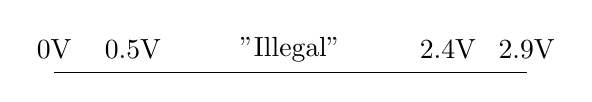
\begin{tikzpicture}
  \node (a) at (0,1) {0V};
  \node (b) at (1,1) {0.5V};
  \node (c) at (5,1) {2.4V};
  \node (d) at (6,1) {2.9V};
  \node (b) at (3,1) {"Illegal"};
  \draw (0,.7) -- (6,.7);
\end{tikzpicture}
\raggedright

\end{document}
